%-------------------------------------------------------------------------------
% EVALUATING CONCEPTS RATHER THAN ATTRIBUTES
%-------------------------------------------------------------------------------
\subsection{Abstraction}
\begin{frame}{What FCA brings to the table}{Abstraction}
\begin{figure}[ht]
\begin{minipage}[t]{0.55\linewidth}
\vspace{0pt}
\centering
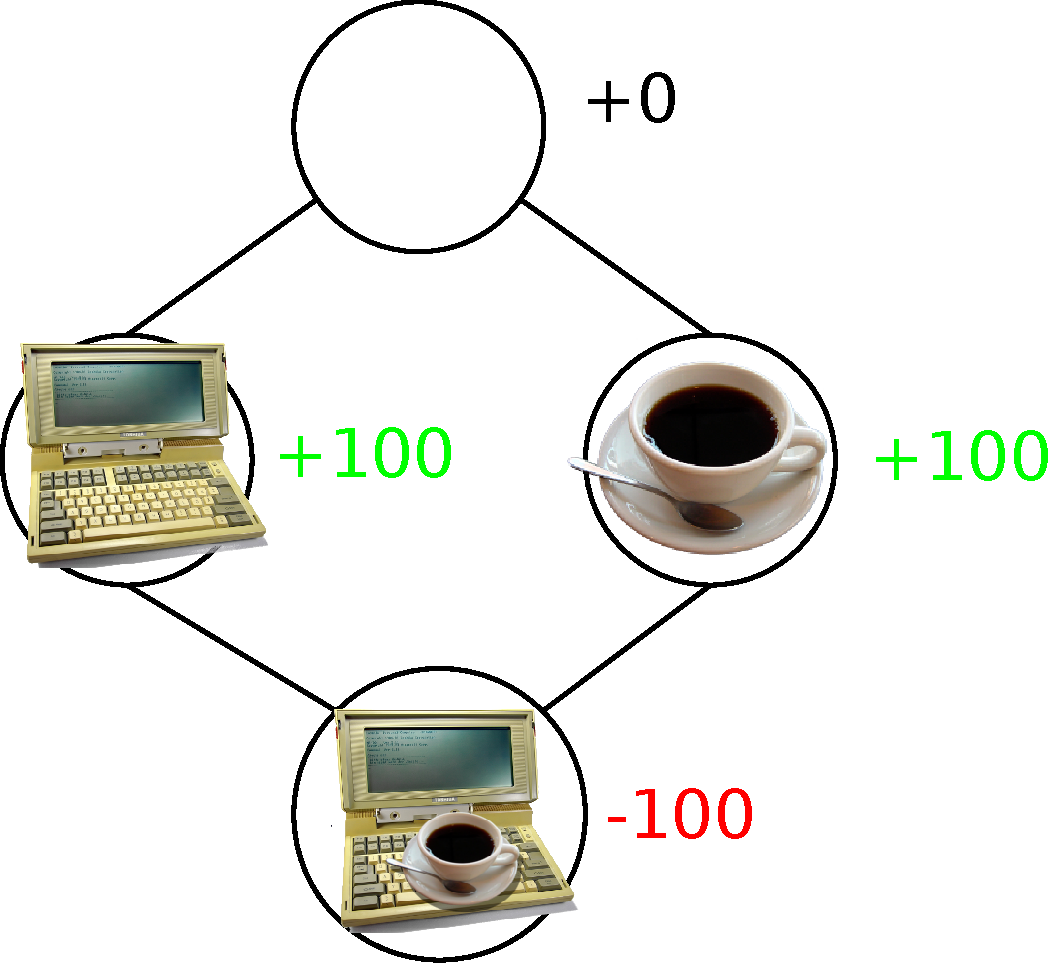
\includegraphics[width=\textwidth]{img/introduction/fca_coffee.pdf}
\end{minipage}
\hfill
\begin{minipage}[t]{0.40\linewidth}
\vspace{0pt}
\begin{block}{To reiterate\ldots}
\begin{itemize}
\item object nodes,
\item attribute nodes,
\item \underline{composite nodes},
\item \underline{abstract nodes}.
\end{itemize}
\vspace{0.4cm}
Evaluate concepts, not just objects and attributes.
\end{block}
\end{minipage}
\end{figure}

\end{frame}

%-------------------------------------------------------------------------------
% ELIMINATION OF REDUNDANCY
%-------------------------------------------------------------------------------
\subsection{Reducing redundancy}
\begin{frame}{What FCA brings to the table}{Reducing redundancy}

\begin{itemize}
\item Attributes always found together can be merged,
\item<2-> beware of introducing errors!
\end{itemize}

\begin{figure}[ht]
  \begin{minipage}[t]{0.3\linewidth}
    \vspace{0pt}
    \centering
    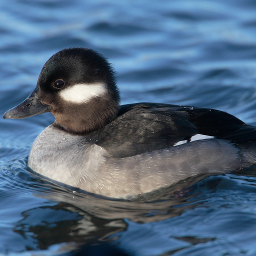
\includegraphics[width=\textwidth]{img/fca/duck1}
    \\ \color{green}{\footnotesize $hasBill(x) \wedge isDuck(x)$}
  \end{minipage}
  \hfill
  \begin{minipage}[t]{0.3\linewidth}
    \vspace{0pt}
    \centering
    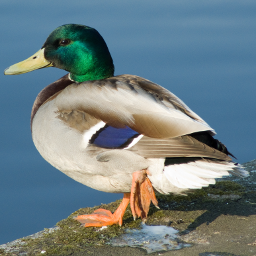
\includegraphics[width=\textwidth]{img/fca/duck2}
    \\ \color{green}{\footnotesize $hasBill(y) \wedge isDuck(y)$}
  \end{minipage}
  \hfill
  \pause
  \begin{minipage}[t]{0.3\linewidth}
    \vspace{0pt}
    \centering
    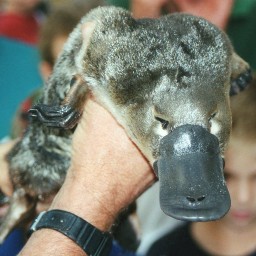
\includegraphics[width=\textwidth]{img/fca/platypus}
    \\ \color{red}{\footnotesize $hasBill(y) \wedge \neg{}isDuck(y)$}
  \end{minipage}
\end{figure}

\end{frame}

\begin{frame}{What FCA brings to the table}{Reducing redundancy}
  \begin{figure}[ht]
    \begin{minipage}[t]{0.8\linewidth}
      \vspace{0pt}
      \centering
      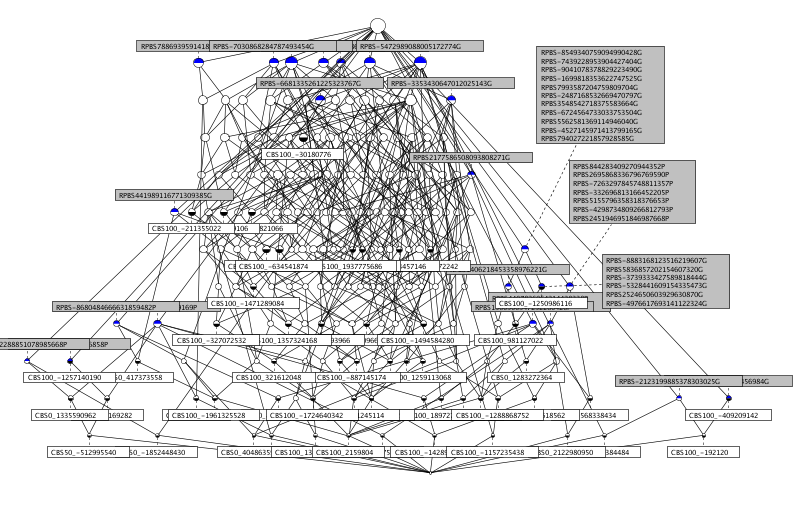
\includegraphics[width=\textwidth]{img/fca/lattice1}
    \end{minipage}
    \hfill
    \begin{minipage}[t]{0\linewidth}
    \end{minipage}
  \end{figure}
\end{frame}


%-------------------------------------------------------------------------------
% FASTER QUERIES
%
%% on peut en dégager une hiérarchie des RPBS. Celle-ci pourrait
%% permettre une recherche plus intelligente des RPBS (réduction du
%% nombre d'homomorphismes à appliquer sur chaque plateau) et donc un
%% gain de temps pour la prise de décision sans devoir réduire
%% drastiquement le nombre de RPBS. On peut imaginer que le système
%% effectuerait une recherche approfondie à posteriori afin de ne pas
%% biaiser l'apprentissage. (L'idée générale est, pendant la phase de
%% jeu, de classer le CBS à évaluer dans un concept et de lui
%% attribuer le point associé à celui-ci. Ce qui permettrait de
%% profiter de la structure du treillis pour diminuer drastiquement le
%% nombre de RPBS rechercher. À savoir que c'est l'étape la plus
%% coûteuse.)
%-------------------------------------------------------------------------------
\subsection{Faster queries}
\begin{frame}{What FCA brings to the table}{Faster queries}

\begin{figure}[ht]
  \begin{minipage}[t]{0.52\linewidth}
    \vspace{0pt}
      \begin{itemize}
      \item Lattice provides partial-order,
      \item prune unnecessary checks,
      \item<2> avoid bias with intermittent extensive searches.
      \end{itemize}
  \end{minipage}
  \hfill
  \begin{minipage}[t]{0.45\linewidth}
    \vspace{0pt}
    \centering
    \includegraphics<1-1>[width=\textwidth]{img/fca/hierarchy1}	
    \includegraphics<2-2>[width=\textwidth]{img/fca/hierarchy2}		
  \end{minipage}
\end{figure}

\end{frame}

\begin{frame}{What FCA brings to the table}{Faster queries}


\begin{figure}[ht]
  \begin{minipage}[t]{0.8\linewidth}
    \vspace{0pt}
    \centering
    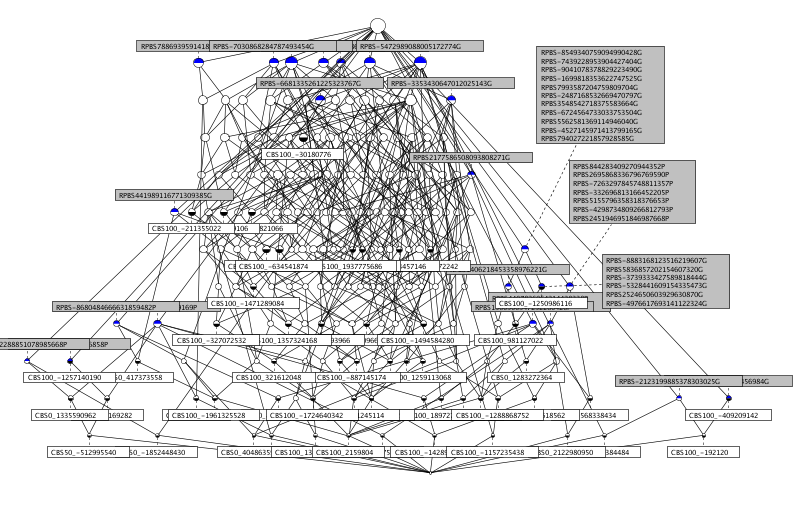
\includegraphics[width=\textwidth]{img/fca/lattice1}
  \end{minipage}
  \hfill
  \begin{minipage}[t]{0\linewidth}

  \end{minipage}
\end{figure}

\end{frame}


%-------------------------------------------------------------------------------
% CHOOSING NEW CONFIGURATIONS 
%
%% Les RPBS introduit dans des concepts
%% parents d'un concept commun (introduisant au moins un CBS), ont
%% potentiellement une sous-partie commune qu'il peut-être intéressant
%% d'extraire comme un nouveau RPBS. (voir common_part.png)
% -------------------------------------------------------------------------------
\subsection{Generating configurations}
\begin{frame}{What FCA brings to the table}{Generating configurations}

\begin{figure}[ht]
  \begin{minipage}[t]{0.45\linewidth}
    \vspace{0pt}
    \centering
    \includegraphics<1-1>[width=\textwidth]{img/fca/ressemble1}	
    \includegraphics<2-2>[width=\textwidth]{img/fca/ressemble2}		
  \end{minipage}
  \hfill
  \begin{minipage}[t]{0.52\linewidth}
    \vspace{0pt}
  \begin{itemize}
    \item The lattice shows attributes instantiated together,
    \item<2> they may well have something in common!
  \end{itemize}
  \end{minipage}
\end{figure}
\end{frame}

\begin{frame}{What FCA brings to the table}{Generating configurations}
  \begin{figure}[ht]
    \begin{minipage}[t]{0.8\linewidth}
      \vspace{0pt}
      \centering
      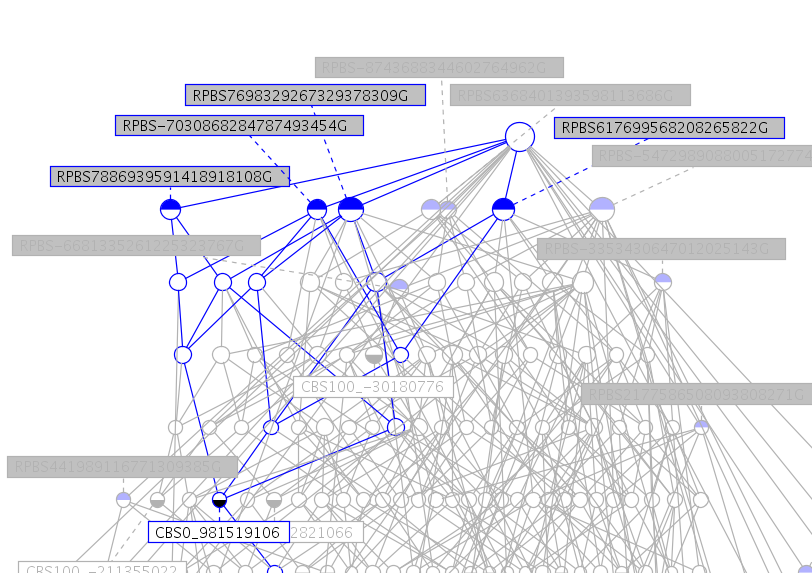
\includegraphics[width=\textwidth]{img/fca/common_part}
    \end{minipage}
    \hfill
    \begin{minipage}[t]{0\linewidth}
    \end{minipage}
  \end{figure}
\end{frame}
